\documentclass[a4paper, 12pt]{article}
\usepackage[utf8]{inputenc}
\usepackage[english, ukrainian]{babel}

\usepackage{amsmath, amssymb}
\usepackage{multicol}
\usepackage{graphicx}
\usepackage{float}

\allowdisplaybreaks
\setlength\parindent{0pt}
\numberwithin{equation}{subsection}

\usepackage{hyperref}
\hypersetup{unicode=true,colorlinks=true,linktoc=all,linkcolor=red}

\numberwithin{equation}{subsection}

\renewcommand{\bf}[1]{\textbf{#1}}
\renewcommand{\it}[1]{\textit{#1}}
\newcommand{\bb}[1]{\mathbb{#1}}
\renewcommand{\cal}[1]{\mathcal{#1}}

\renewcommand{\epsilon}{\varepsilon}
\renewcommand{\phi}{\varphi}

\DeclareMathOperator{\diam}{diam}
\DeclareMathOperator{\rang}{rang}
\DeclareMathOperator{\const}{const}

\newenvironment{system}{%
  \begin{equation}%
    \left\{%
      \begin{aligned}%
}{%
      \end{aligned}%
    \right.%
  \end{equation}%
}
\newenvironment{system*}{%
  \begin{equation*}%
    \left\{%
      \begin{aligned}%
}{%
      \end{aligned}%
    \right.%
  \end{equation*}%
}

\makeatletter
\newcommand*{\relrelbarsep}{.386ex}
\newcommand*{\relrelbar}{%
  \mathrel{%
    \mathpalette\@relrelbar\relrelbarsep%
  }%
}
\newcommand*{\@relrelbar}[2]{%
  \raise#2\hbox to 0pt{$\m@th#1\relbar$\hss}%
  \lower#2\hbox{$\m@th#1\relbar$}%
}
\providecommand*{\rightrightarrowsfill@}{%
  \arrowfill@\relrelbar\relrelbar\rightrightarrows%
}
\providecommand*{\leftleftarrowsfill@}{%
  \arrowfill@\leftleftarrows\relrelbar\relrelbar%
}
\providecommand*{\xrightrightarrows}[2][]{%
  \ext@arrow 0359\rightrightarrowsfill@{#1}{#2}%
}
\providecommand*{\xleftleftarrows}[2][]{%
  \ext@arrow 3095\leftleftarrowsfill@{#1}{#2}%
}
\makeatother

\newcommand{\NN}{\mathbb{N}}
\newcommand{\ZZ}{\mathbb{Z}}
\newcommand{\QQ}{\mathbb{Q}}
\newcommand{\RR}{\mathbb{R}}
\newcommand{\CC}{\mathbb{C}}

\newcommand{\Max}{\displaystyle\max\limits}
\newcommand{\Sup}{\displaystyle\sup\limits}
\newcommand{\Sum}{\displaystyle\sum\limits}
\newcommand{\Int}{\displaystyle\int\limits}
\newcommand{\Iint}{\displaystyle\iint\limits}
\newcommand{\Lim}{\displaystyle\lim\limits}

\newcommand*\diff{\mathop{}\!\mathrm{d}}

\newcommand*\rfrac[2]{{}^{#1}\!/_{\!#2}}


\title{{\Huge МАТЕМАТИЧНА ФІЗИКА}}
\author{Скибицький Нікіта}
\date{\today}

\usepackage{amsthm}
\usepackage[dvipsnames]{xcolor}
\usepackage{thmtools}
\usepackage[framemethod=TikZ]{mdframed}

\theoremstyle{definition}
\mdfdefinestyle{mdbluebox}{%
	roundcorner = 10pt,
	linewidth=1pt,
	skipabove=12pt,
	innerbottommargin=9pt,
	skipbelow=2pt,
	nobreak=true,
	linecolor=blue,
	backgroundcolor=TealBlue!5,
}
\declaretheoremstyle[
	headfont=\sffamily\bfseries\color{MidnightBlue},
	mdframed={style=mdbluebox},
	headpunct={\\[3pt]},
	postheadspace={0pt}
]{thmbluebox}

\mdfdefinestyle{mdredbox}{%
	linewidth=0.5pt,
	skipabove=12pt,
	frametitleaboveskip=5pt,
	frametitlebelowskip=0pt,
	skipbelow=2pt,
	frametitlefont=\bfseries,
	innertopmargin=4pt,
	innerbottommargin=8pt,
	nobreak=true,
	linecolor=RawSienna,
	backgroundcolor=Salmon!5,
}
\declaretheoremstyle[
	headfont=\bfseries\color{RawSienna},
	mdframed={style=mdredbox},
	headpunct={\\[3pt]},
	postheadspace={0pt},
]{thmredbox}

\declaretheorem[style=thmbluebox,name=Теорема,numberwithin=subsubsection]{theorem}
\declaretheorem[style=thmbluebox,name=Лема,numberwithin=subsubsection]{lemma}
\declaretheorem[style=thmbluebox,name=Твердження,numberwithin=subsubsection]{proposition}
\declaretheorem[style=thmbluebox,name=Принцип,numberwithin=subsubsection]{th_principle}
\declaretheorem[style=thmbluebox,name=Закон,numberwithin=subsubsection]{law}
\declaretheorem[style=thmbluebox,name=Закон,numbered=no]{law*}
\declaretheorem[style=thmbluebox,name=Формула,numberwithin=subsubsection]{th_formula}
\declaretheorem[style=thmbluebox,name=Рівняння,numberwithin=subsubsection]{th_equation}
\declaretheorem[style=thmbluebox,name=Умова,numberwithin=subsubsection]{th_condition}
\declaretheorem[style=thmbluebox,name=Наслідок,numberwithin=subsubsection]{corollary}

\declaretheorem[style=thmredbox,name=Приклад,numberwithin=subsubsection]{example}
\declaretheorem[style=thmredbox,name=Приклади,sibling=example]{examples}

\declaretheorem[style=thmredbox,name=Властивість,numberwithin=subsubsection]{property}
\declaretheorem[style=thmredbox,name=Властивості,sibling=property]{properties}

\mdfdefinestyle{mdgreenbox}{%
	skipabove=8pt,
	linewidth=2pt,
	rightline=false,
	leftline=true,
	topline=false,
	bottomline=false,
	linecolor=ForestGreen,
	backgroundcolor=ForestGreen!5,
}
\declaretheoremstyle[
	headfont=\bfseries\sffamily\color{ForestGreen!70!black},
	bodyfont=\normalfont,
	spaceabove=2pt,
	spacebelow=1pt,
	mdframed={style=mdgreenbox},
	headpunct={ --- },
]{thmgreenbox}

\mdfdefinestyle{mdblackbox}{%
	skipabove=8pt,
	linewidth=3pt,
	rightline=false,
	leftline=true,
	topline=false,
	bottomline=false,
	linecolor=black,
	backgroundcolor=RedViolet!5!gray!5,
}
\declaretheoremstyle[
	headfont=\bfseries,
	bodyfont=\normalfont\small,
	spaceabove=0pt,
	spacebelow=0pt,
	mdframed={style=mdblackbox}
]{thmblackbox}

\declaretheorem[name=Вправа,numberwithin=subsubsection,style=thmblackbox]{exercise}
\declaretheorem[name=Зауваження,numberwithin=subsubsection,style=thmgreenbox]{remark}
\declaretheorem[name=Визначення,numberwithin=subsubsection,style=thmblackbox]{definition}

\newtheorem{problem}{Задача}[subsection]
\newtheorem{sproblem}[problem]{Задача}
\newtheorem{dproblem}[problem]{Задача}
\renewcommand{\thesproblem}{\theproblem$^{\star}$}
\renewcommand{\thedproblem}{\theproblem$^{\dagger}$}
\newcommand{\listhack}{$\empty$\vspace{-2em}} 

\theoremstyle{remark}
\newtheorem*{solution}{Розв'язок}


\begin{document}

\tableofcontents

\setcounter{section}{3}
\setcounter{subsection}{1}
\setcounter{subsubsection}{4}
\setcounter{theorem}{15}
\setcounter{equation}{57}

\subsection{Математичні моделі теорії пружності}

Відомо, що в природі існують пружні тіла, які можуть змінювати свою форму під дією прикладеної сили, а після припинення дії зовнішньої сили приймати початкову форму. Зовнішня сила викликає в пружних тілах:
\begin{itemize}
	\item деформації;
	\item напруження.
\end{itemize}

\begin{definition}[деформації]
	\it{Деформацією} називають зміну положення одних точок тіла відносно інших.
\end{definition}

\begin{definition}[напружень]
	\it{Напруженнями} називають внутрішні сили, які прагнуть повернути тіло в положення рівноваги.
\end{definition}

\begin{definition}[математичної моделі теорії пружності]
	\it{Математична модель теорії пружності} --- це система диференціальних рівнянь, які описують кількісний зв'язок між зміною форми тіла (деформаціями) і внутрішніми зусиллями (напруженнями). 
\end{definition}

Введемо позначення:
\begin{itemize}
	\item $x$, $y$, $z$ --- координати точки у просторі;
 	\item $U(x, y, z, t)$, $V(x, y, z, t)$, $W(x, y, z, t)$ --- координати \it{вектора зміщень} в напрямку вісей $Ox$, $Oy$, $Oz$ відповідно.

 	\begin{remark}
 		\it{Вектор зміщень} показує зміщення точки тіла з координатами $x$, $y$, $z$ в напрямку однієї з координатних вісей в момент часу $t$ від положення рівноваги
 	\end{remark}

	\item $F_x(x, y, z, t)$, $F_y(x, y, z, t)$, $F_z(x, y, z, t)$ --- компоненти \it{вектора поверхневих сил} в напрямку вісей $Ox$, $Oy$, $Oz$ відповідно.

	\begin{remark}
		\it{Вектор поверхневих сил} показує які сили діють на поверхню тіла.
	\end{remark}

	\item $X(x, y, z, t)$, $Y(x, y, z, t)$, $Z(x, y, z, t)$ --- вектори \it{об'ємних сил};
	\item $\diff G$ --- елемент об'єму; $\diff S$ --- елемент поверхні.
\end{itemize}

Розглянемо просту фізичну модель взаємодії між собою двох частин пружного тіла. Нехай прямокутний паралелепіпед з нескінченно малим поперечним перерізом $\diff y \times \diff z$ витягнутий вздовж вісі $x$ та умовно розділений на дві частини площиною ортогональною вісі $x$:
\begin{figure}[H]
	\centering
	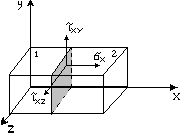
\includegraphics[]{img/8-1.png}
\end{figure}

Охарактеризуємо силу з якою правий паралелепіпед діє на лівий паралелепіпед через переріз $\diff y \times \diff z$ в площині $yOz$ (на рис. площина взаємодії виділена сірим кольором). \medskip

Нехай $\bf{t}^{(x)} = \left( \sigma_x, \tau_{xy}, \tau_{xz} \right)$ --- \it{вектор сили}.

\begin{definition}[вектора сили]
	\it{Вектор сили} показує, з якою силою (на одиницю поверхні) правий паралелепіпед діє на лівий паралелепіпед.
\end{definition}

\begin{remark}
	При цьому $\sigma_x$ --- компонента, що може стискати, або розтягувати лівий паралелепіпед, $\tau_{xy}$, $\tau_{xz}$ --- компоненти, що стискають паралелепіпед в напрямках вісей $Oy$ та $Oz$ відповідно.
\end{remark}

Аналогічно, для паралелепіпедів витягнутих вздовж вісей $Oy$ та $Oz$ можна розглянути сили, яки діють в двох інших площинах $xOz$ та $xOy$ на одиницю площі цих перерізів та охарактеризувати їх векторами:
\begin{align}
	\bf{t}^{(y)} &= \left( \tau_{yx}, \sigma_y, \tau_{yz} \right), \\
	\bf{t}^{(z)} &= \left( \tau_{zx}, \tau_{zy}, \sigma_z \right).
\end{align}

Для будь-якого паралелепіпеда з довжиною ребер $\diff x$, $\diff y$, $\diff z$ а тим самим точки простору напружений стан тіла можна охарактеризувати матрицею
\begin{equation}
	\label{eq:3.2.3}
	\begin{pmatrix}
		\sigma_x & \tau_{xy} & \tau_{xz} \\
		\tau_{yx} & \sigma_y & \tau_{yz} \\
		\tau_{zx} & \tau_{zy} & \sigma_z
	\end{pmatrix}
\end{equation}

\begin{remark}
	При розгляді моделі взаємодії правого паралелепіпеда та лівого паралелепіпеда через спільний переріз має місце принцип рівнодії та протидії, тобто сила, з якою правий паралелепіпед діє на лівий паралелепіпед рівна за величиною та протилежна за напрямком силі з якою лівий паралелепіпед діє на правий паралелепіпед. Сили, що діють на тіло обираються зі знаком плюс, якщо вони діють на переріз, який обмежує тіло з боку зростання значення координатної вісей і зі знаком мінус, якщо вони діють на поверхню, що обмежує тіло з боку спадання значень координатних вісей.
\end{remark}

\subsubsection{Закони рівноваги елемента поверхні}

Розглянемо елементарну модель пружної взаємодії. Нехай всередині пружного тіла ми виділили нескінченно малий тетраедр $OABC$, $\vec n$ --- вектор зовнішньої нормалі до грані $ABC$, а $S$ --- площа цієї грані:
\begin{figure}[H]
	\centering
	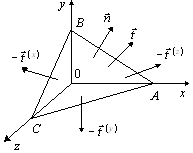
\includegraphics[]{img/8-2.png}
\end{figure}

Нехай $\vec f = (f_x, f_y, f_z)$ --- вектор поверхневої сили, що діє на одиницю площі грані $ABC$. \medskip

Вектор нормалі
\begin{equation}
	\vec{\bf{n}} = \big( \cos\left( \vec n, x \right), \cos \left( \vec n, y \right), \cos \left( \vec n, z \right) \big),
\end{equation}
а
\begin{equation}
	S \cdot \cos \left(\vec n, x \right), \quad S \cdot \cos \left(\vec n, y \right), \quad S \cdot \cos \left(\vec n, z \right) 	
\end{equation} 
--- площі граней тетраедра, ортогональних вісям $Ox$, $Oy$, $Oz$. \medskip

Якщо тетраедр знаходиться в стані спокою, або рівномірного прямолінійного руху, то рівнодіюча сил, що діють на всі чотири грані дорівнює нулю, тобто: 
\begin{equation}
	\vec f \cdot S - \bf{t}^{(x)} \cdot S \cdot \cos \left( \vec n, x\right) - \bf{t}^{(y)} \cdot S \cdot \cos \left( \vec n, y\right) - \bf{t}^{(z)} \cdot S \cdot \cos \left( \vec n, z\right) = 0.
\end{equation}

Після скорочення на $S$ отримаємо
\begin{theorem}[векторна форма закону рівноваги елемента поверхні]
	Виконується співвідношення:
	\begin{equation}
		\vec f = \bf{t}^{(x)} \cdot \cos \left( \vec n, x\right) + \bf{t}^{(y)} \cdot \cos \left( \vec n, y\right) + \bf{t}^{(z)} \cdot \cos \left( \vec n, z\right).
	\end{equation}
\end{theorem}

Запишемо закон рівноваги елемента поверхні в скалярному вигляді:
\begin{align}
	\sigma_x \cdot \cos \left( \vec n, x \right) + \tau_{xy} \cdot \cos \left( \vec n, y \right) + \tau_{xz} \cdot \cos \left( \vec n, z \right) &= f_x, \\
	\tau_{yx} \cdot \cos \left( \vec n, x \right) + \sigma_y \cdot \cos \left( \vec n, y \right) + \tau_{yz} \cdot \cos \left( \vec n, z \right) &= f_y, \\
	\tau_{zx} \cdot \cos \left( \vec n, x \right) + \tau_{zy} \cdot \cos \left( \vec n, y \right) + \sigma_z \cdot \cos \left( \vec n, z \right) &= f_z.
\end{align}

У випадку, коли елементарний трикутник $ABC$ є частиною реальної зовнішньої поверхні тіла, то закон рівноваги елемента поверхні приймає вигляд:
\begin{align}
	\sigma_x \cdot \cos \left( \vec n, x \right) + \tau_{xy} \cdot \cos \left( \vec n, y \right) + \tau_{xz} \cdot \cos \left( \vec n, z \right) &= F_x, \\
	\tau_{yx} \cdot \cos \left( \vec n, x \right) + \sigma_y \cdot \cos \left( \vec n, y \right) + \tau_{yz} \cdot \cos \left( \vec n, z \right) &= F_y, \\
	\tau_{zx} \cdot \cos \left( \vec n, x \right) + \tau_{zy} \cdot \cos \left( \vec n, y \right) + \sigma_z \cdot \cos \left( \vec n, z \right) &= F_z,
\end{align}
де $(F_x, F_y, F_z)$ --- вектор поверхневих сил. \medskip

\subsubsection{Закон рівноваги елемента об'єму}

Розглянемо будь-який об'єм $G$ та його елементарний об'єм $\diff G$. \medskip

Об'ємні сили, що діють на тіло об'єму $G$ можна обчислити у вигляді
\begin{equation}
	\Iiint_G \begin{pmatrix} X \\ Y \\ Z \end{pmatrix} \diff G.
\end{equation}

Через будь-яку елементарну поверхню тіла діє поверхнева сила $\vec f \cdot \diff S$, а результуюча поверхнева сила, яка діє на тіло через усю поверхню $S$, що обмежує тіло має вигляд 
\begin{equation}
	\Iint_S \vec f \diff S,
\end{equation}
або, в скалярному вигляді:
\begin{equation}
	\Iint_S \left( \bf{t}^{(x)} \cdot \cos \left( \vec n, x \right) + \bf{t}^{(y)} \cdot \cos\left(\vec n, y\right) + \bf{t}^{(z)} \cdot \cos \left(\vec n, z\right) \right) \diff S.
\end{equation}

\begin{theorem}[векторний запис закону рівноваги елементу об'єму]
	Для того щоб тіло знаходилося в стані спокою або рухалось рівномірно і прямолінійно, рівнодіюча об'ємної та поверхневої сил повинна дорівнювати нулю:
	\begin{multline}
		\Iint_S \big( \bf{t}^{(x)} \cos(\vec n, x) + \bf{t}^{(y)} \cos(\vec n, y) + \bf{t}^{(z)} \cos(\vec n, z) \big) \diff S + \\ 
		+ \Iiint_G \begin{pmatrix} X \\ Y \\ Z \end{pmatrix} \diff G = 0.
	\end{multline}
\end{theorem}

\begin{theorem}[скалярний запис закону рівноваги елементу об'єму]
	\begin{system}
		\Iint_S \left( \sigma_x \cos(\vec n, x) + \tau_{yx} \cos(\vec n, y) + \tau_{zx} \cos(\vec n, z)\right) \diff S + \Iiint_G X \diff G &= 0, \\
		\Iint_S \left( \tau_{xy} \cos(\vec n, x) + \sigma_y \cos(\vec n, y) + \tau_{zy} \cos(\vec n, z)\right) \diff S + \Iiint_G Y \diff G &= 0, \\
		\Iint_S \left( \tau_{xz} \cos(\vec n, x) + \tau_{yz} \cos(\vec n, y) + \sigma_z \cos(\vec n, z)\right) \diff S + \Iiint_G Z \diff G &= 0.
	\end{system}
\end{theorem}

\begin{remark}
	Додатковою умовою рівноважного положення тіла окрім закону рівноваги елементу об'єму є виконання закону збереження моментів сил з якого випливає симетричність матриці \eqref{eq:3.2.3}:
	\begin{equation}
		\tau_{x y} = \tau_{y x}, \quad \tau_{x z} = \tau_{z x}, \quad \tau_{y z} = \tau_{z y}.
	\end{equation}
\end{remark}

Враховуючи факт симетрії, останній закон можна записати у вигляді
\begin{system}
	\Iint_S \left( \bf{t}^{(x)}, \vec n\right) \diff S + \Iiint_G X \diff G &= 0, \\
	\Iint_S \left( \bf{t}^{(y)}, \vec n\right) \diff S + \Iiint_G Y \diff G &= 0, \\
	\Iint_S \left( \bf{t}^{(z)}, \vec n\right) \diff S + \Iiint_G Z \diff G &= 0.
\end{system}
де 
\begin{equation}
	\vec{\bf{n}} = \big( \cos(\vec n, x), \cos(\vec n, y), \cos(\vec n, z) \big)
\end{equation}
--- вектор зовнішньої нормалі до поверхні. \medskip

Враховуючи формулу Остроградського-Гауса, кожен поверхневий інтеграл перетворимо в об'ємний, в результаті отримаємо
\begin{theorem}[диференціальна форма запису закону рівноваги елементу об'єму]
	Виконуються співвідношення:
	\begin{system}
		\Iiint_G \left( \nabla \cdot \bf{t}^{(x)} + X \right) \diff G &= 0, \\
		\Iiint_G \left( \nabla \cdot \bf{t}^{(y)} + Y \right) \diff G &= 0, \\
		\Iiint_G \left( \nabla \cdot \bf{t}^{(z)} + Z \right) \diff G &= 0.
	\end{system}
\end{theorem}

\begin{definition}[тензора напружень]
	В подальшому симетричну матрицю \eqref{eq:3.2.3} будемо називати \it{тензором напружень}.
\end{definition}

\subsubsection{Тензор напружень, головні вісі тензора напружень}

Позначимо через   орти прямокутної система координат з координатними осями  . 
Введемо нову систему координат з ортами  . та осями  .
З'ясуємо, яким чином пов'язані вектори  , які складають стрічки (стовпці) тензору напружень у системі координат  , з векторами  , які складають стрічки (стовпці) тензору напружень у новій системі координат  .
Згідно до загальних формул переходу від одного ортогонального базису до іншого, можна записати:
   			(2.8).
Координати ортів нової системи координат мають значення:
 
 
 
Для знаходження будь --- якої компоненти тензора напружень  , необхідно обчислити скалярний добуток  . Так, наприклад,    .
Отже, для довільної компоненти тензора напружень має місце формула переходу від однієї до іншої системи координат 
 								(2.9). 
У формулі (2.9) використані позначення 	 . 
Таким чином, тензор напружень --- це симетрична матриця,  , компоненти якої перетворюються за формулою (2.9) при переході до нової прямокутної системи координат. 
Поставимо задачу вибору нової прямокутної системи координат, для якої тензор напружень має діагональну форму. Нехай   - орти нової прямокутної системи координат. Для того, щоб тензор   мав діагональну форму запису, кожен вектор  ,   в новій системі координат повинен бути колінеарним відповідному орту   ,  тобто  . 
Скористаємось формулою (2.8) та запишемо співвідношення для пошуку ортів  ;
Запишемо останнє співвідношення в координатному вигляді:
 			 (2.10).
Для ортонормованого базису 	 .
В матрично --- векторній формі (2.10) має вигляд
 . 										(2.10').
Ця задача на власні значення з симетричною матрицею має три дійсних власних числа, позначимо їх  , тобто  , і три ортонормовані власні вектори  .
Координатні вісі, для яких тензор напружень має діагональний вигляд, називаються головними вісями тензора напружень.
Відповідні діагональні компоненти тензора напружень  ,   називаються головними компонентами тензора напружень. 
Використовуючи формулу (2.9), запишемо зв'язок між компонентами тензора напружень в декартових координатах   і головними компонентами тензора напружень:
  							(2.11), 
 	 					(2.11/).

\subsubsection{Тензор деформацій і закони його перетворення}

Раніше були введені характеристики:   --зміщення точки з координатами (x, y, z) від положення рівноваги в напрямку відповідної вісі.
Розглянемо можливі види деформації.
1. Нормальні деформації - (зміна довжини в напрямку координатної вісі) характеризуються відносною зміною довжини відрізків.
Приклавши силу в напрямку вісі  , точка   змістилася і зайняла положення  ; точка   теж змістилася і зайняла положення   .
Порахуємо відносне подовження відрізка   після прикладення до нього напруження:
 .
Аналогічно, можна ввести характеристику відносного подовження в напрямку двох інших вісей. 
Отже, нормальні деформації характеризуються частинними похідними  .
2. Зрізуючи (дотичні) деформації  будемо характеризувати абсолютною зміною кутів між відрізками в кожній з трьох координатних площин, які до початку дії напружень були ортогональними. 
Розглянемо наступну фізичну модель. Нехай відрізки   та   довжини   та   відповідно після дії прикладених сил зайняли положення   та   відповідно. Точка   змістилася на відстань  , а точка   змістилася на відстань  .
Тоді    .
Аналогічно   .
Сумарна зміна кута  . Позначимо   .
Провівши аналогічні міркування щодо інших координатних площин отримаємо: 
 ,	 				(2.12).
Позначимо:  , , , ,			(2.13).
В результаті повну деформацію у будь --- якій точці простору можна охарактеризувати симетричною матрицею:  , яка називається симетричним тензором деформацій.

\subsubsection{Перетворення тензора деформацій до нових прямокутних координат}

Вивчимо перетворення симетричного тензору деформацій при переході від однієї прямокутної системи координат до іншої. Нехай   вісі нової системи координат (замість  ), а функції   зміщення в напряму нових вісей.
Враховуючи формули переходу від одного ортогонального базису до іншого можемо записати:
  
  					(2.12),
 
  
  
  
 					(2.13).
  
 
У формулах (2.12), (2.13)   координати ортів нового базису.
Знайдемо вирази для компонентів тензору у новій системі координатах:   при  .
Зокрема для   отримаємо:
     
Розкриваючи дужки і використовуючи відповідні позначення отримаємо наступну формулу: 	 .
Загальна формула перетворення тензора деформацій матиме вигляд:
 ,  			(2.14).

\end{document}